\section{Interface (api)}

\begin{figure}[htp]
\center
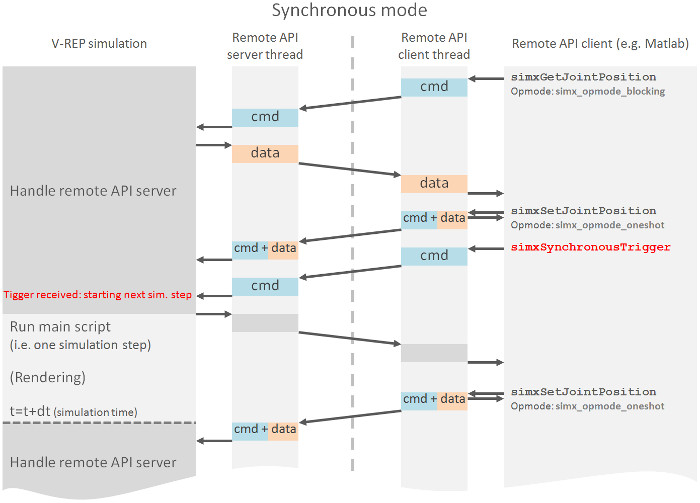
\includegraphics[width=0.6\textwidth]{figures/remoteApiSynchronous}
\caption{Synchronous operation mode explanation}
\label{fig:remoteApi}
\end{figure}

\section{First simple simulations}

\section{Robot design}

The final dimensions of the robot respect the rules of the contest:
\begin{itemize}
\item Height : $61.3cm$
\item Height of COM : $34cm$
\item Height of legs : $cm$
\item Height max is $< 1.5 \times 61.3$.
\item Foot area is $ cm^2$.
\end{itemize} 

\section{Application : stand up routines}
This section is heavily inspired by \cite{Stuckler06}